\section{Architectural Modelling in SysML}
\label{sec:sysml}
To illustrate the approach, we take an example (water tank) inspired by \cite{AmalioPCW16}. According to the I/O dependency information between the FMUs, the architectural model for water tank is constructed using SysML.
\subsection{Case Study: Water Tank}

The water tank system, as shown in Fig.\ref{wts-sm}, is our running example. A source of water flows into the water tank whose water flows into the drain, and the source is controlled by a valve; when the valve is open the water flows into the water tank. The valve, managed by a software controller, is opened or closed stochastically or depending on the water level. There are two variants of water tank system depending on the various connections between controller, valve and tank. 

Figure~\ref{wts-fc} is the architecture connection of water tank. There are three connection cases between the FMUs. The first case contains three FMU components (\emph{Controller}, \emph{Valve} and \emph{ Tank1}) and two channels($v \_ vin$, $w \_ win$). The controller and valve are connected with channel $v \_ vin$. The valve and tank1 are connected with channel $w \_ win$. For the second case, there could be a channel $sout \_ s$ between tank1 and controller, which means the water level of tank1 affecting the control strategy of the controller. It is denoted with the gray line. Besides, there could be another tank2 (the gray box). The tank1 and tank2 are connected by the channel $w \_ out$. The orchestration of FMUs for water tank is modeled with SysML block diagram in the next subsection.
\begin{figure}[htbp]
\centering{
		\subfigure[Sketch map of water tank system]{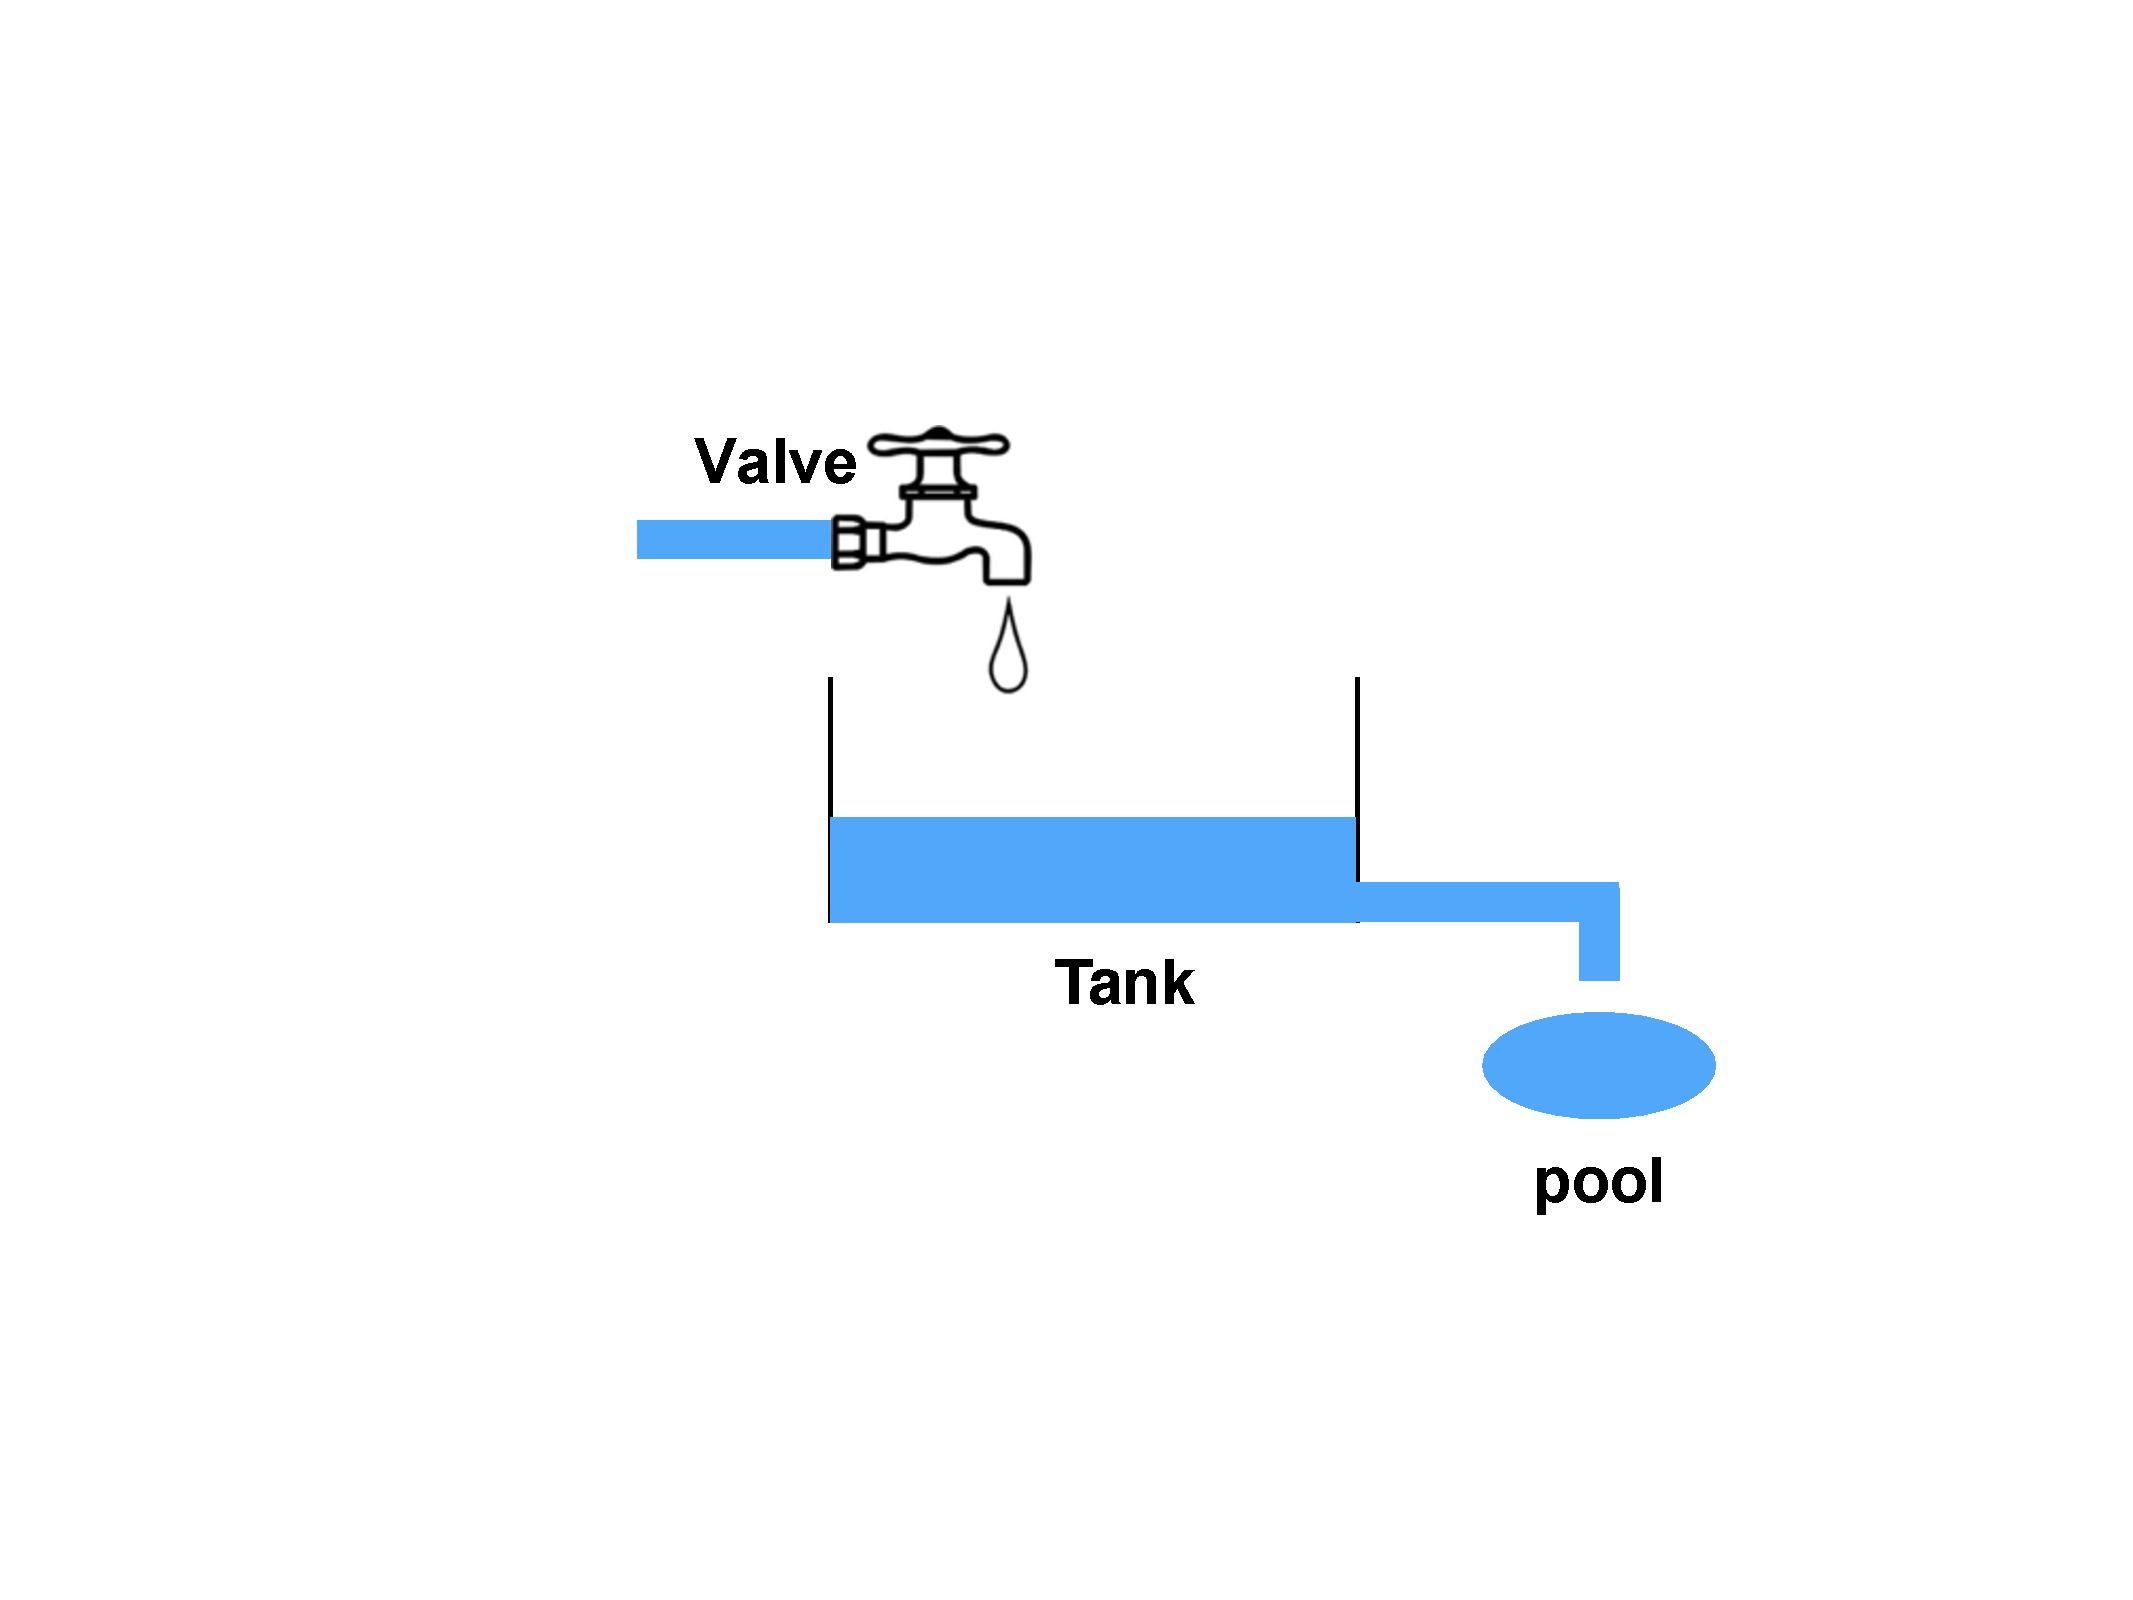
\includegraphics[width=1.2in,height=1.0in]{fig/tank-fig.pdf}
			\label{wts-sm}}
		\hfil
		\subfigure[FMUs connection of water tank system.]{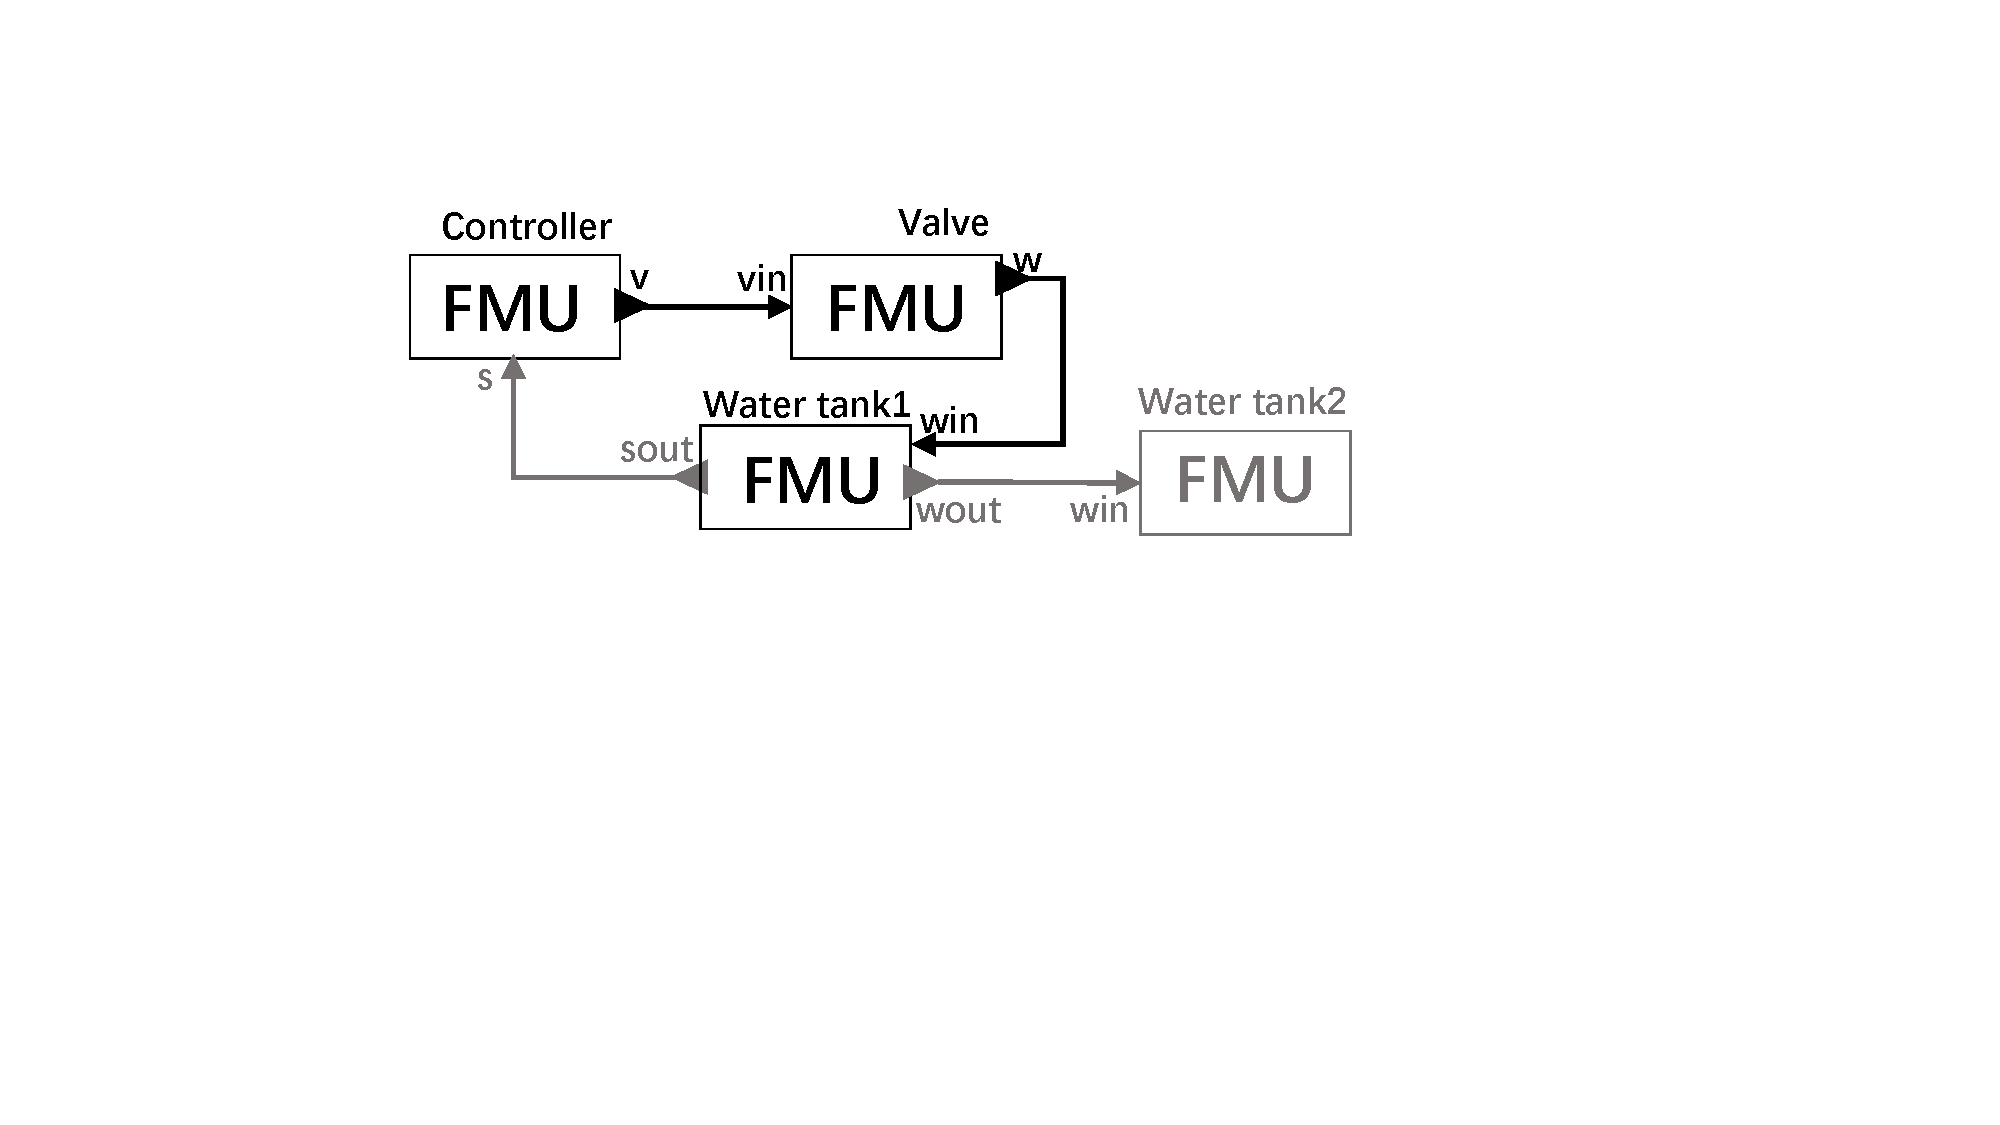
\includegraphics[width=2.0in,height=0.8in]{fig/tank-fra.pdf}
			\label{wts-fc}}
	\caption{Water tank system.}
	\label{wts}
	}
\end{figure}
\subsection{Architecture Modelling in SysML}

\begin{figure*}[htbp]
\centering{
		\subfigure[SysML BDD]{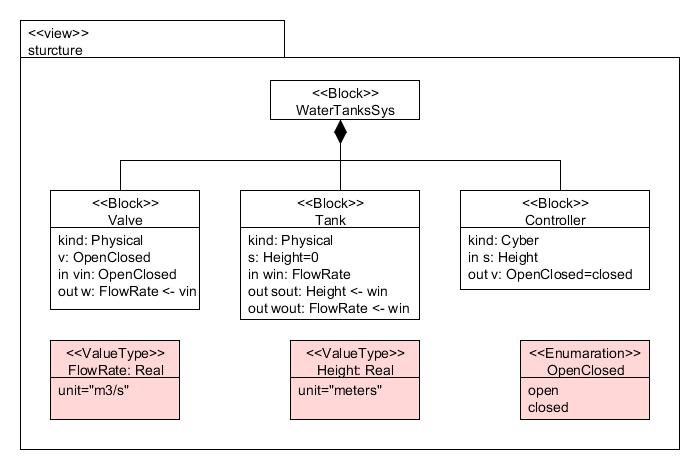
\includegraphics[width=3.2in,height=2.3in]{fig/AD.jpg}
			\label{trs}}
		\hfil
		\subfigure[SysML CD]{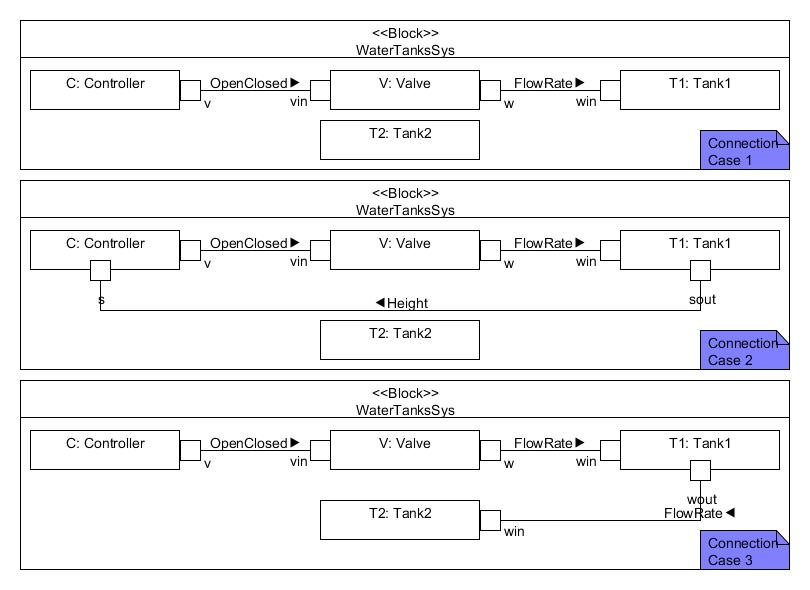
\includegraphics[width=3.2in,height=2.3in]{fig/CD.jpg}
			\label{seq}}
	\caption{The SysML block diagrams for water tank system.}
	\label{trs-seq}
	}
\end{figure*}

SysML is a general purpose domain-specific language (DSL) \cite{SemerathBHSV17} for model-based systems engineering (MBSE) \cite{Dori16}, which is originated as an initiative of the International Council on Systems Engineering (INCOSE) \cite{Pepper2015International} in January 2001. SysML is implemented as a UML profile. The \textit{Block Definition Diagram }(BDD) describes the system blocks and their features (structural and behavioural). The\textit{ Connection Diagram} (CD) describes the internal structure of blocks. The ports of blocks are connected by the connector. The I/O dependence of blocks describes the communication between blocks. SysML block diagrams are usually used to describe the architecture of systems.

Figure~\ref{trs} shows the block definition diagram for the water tank system. The system consists of three blocks, i.e., \emph{Valve}, \emph{Tank} and \emph{Controller}, in which \emph{Valve} and \emph{Tank} are physical components. \emph{Controller} is the cyber component. Each component has its own input and output. For instance, the input interface of \emph{Valve} is named as \emph{vin}, which is used to input the \emph{Open-Closed} signal. 

Figure~\ref{seq} shows the connection diagram for the system. There are three cases for connections. The first case is that the system has one valve, one controller and one tank. The controller sends stochastic signals to control the valve on/off leading to various rate of water flow. The second case is that the signal from the controller is affected by the water level of the tank. The last case is on the basis of the first case and adds another tank2 which is affected by the flow rate of the tank1. How can we assure the correctness of the architecture models? We attempt to verify it with model checking based on timed automata. More details on verification process can be found in the next section.